\section{Versioning avec Git et GitLab}\label{sec:versioning-git-gitlab}

Dans l'entreprise, les équipes de développement utilisent Git pour la gestion des versions et GitLab pour gérer le processus de développement.

Git est un système de gestion de version décentralisé largement utilisé dans le développement de logiciels. Il permet aux équipes de collaborer efficacement sur des projets en suivant les modifications apportées aux fichiers au fil du temps. Grâce à Git, les développeurs peuvent créer des branches pour travailler sur des fonctionnalités spécifiques ou des corrections de bugs sans perturber le code principal. Les commits, qui représentent des enregistrements de changements, sont la pierre angulaire de Git, permettant de garder une trace claire de l'évolution du code.

GitLab, quant à lui, est une plateforme de gestion de développement logiciel basée sur Git. Elle offre un environnement complet pour le cycle de vie du développement, de la planification à la surveillance. GitLab permet aux équipes de suivre les problèmes, de planifier les sprints, de gérer les demandes d'extraction et de créer des pipelines d'intégration continue pour automatiser les tests et le déploiement. En regroupant toutes ces fonctionnalités au même endroit, GitLab facilite la collaboration entre les membres de l'équipe et permet une gestion transparente et efficace des projets de développement.

Parmi ces nombreuses fonctionnalités, les équipes de DevOps et de développement n'utilisent cependant pas les fonctionnalités de gestion de projet et d'intégration continue/de livraison continue de GitLab, puisqu'elles utilisent Jira (comme nous l'avons vu dans la section précédente) et TeamCity (comme nous le verrons dans la section suivante) à ces fins. GitLab est donc principalement utilisé comme un hébergeur de dépôt de code et un outil de révision de code avec des fonctionnalités telles que les demandes de fusion (merge request).

La Figure~\ref{fig:versioning-and-environments} illustre les principes du versioning et les différents environnements utilisés pour héberger les différentes versions du code. Le tableau Y apporte quelques compléments d'information.

\begin{sidewaysfigure}
    \centering
    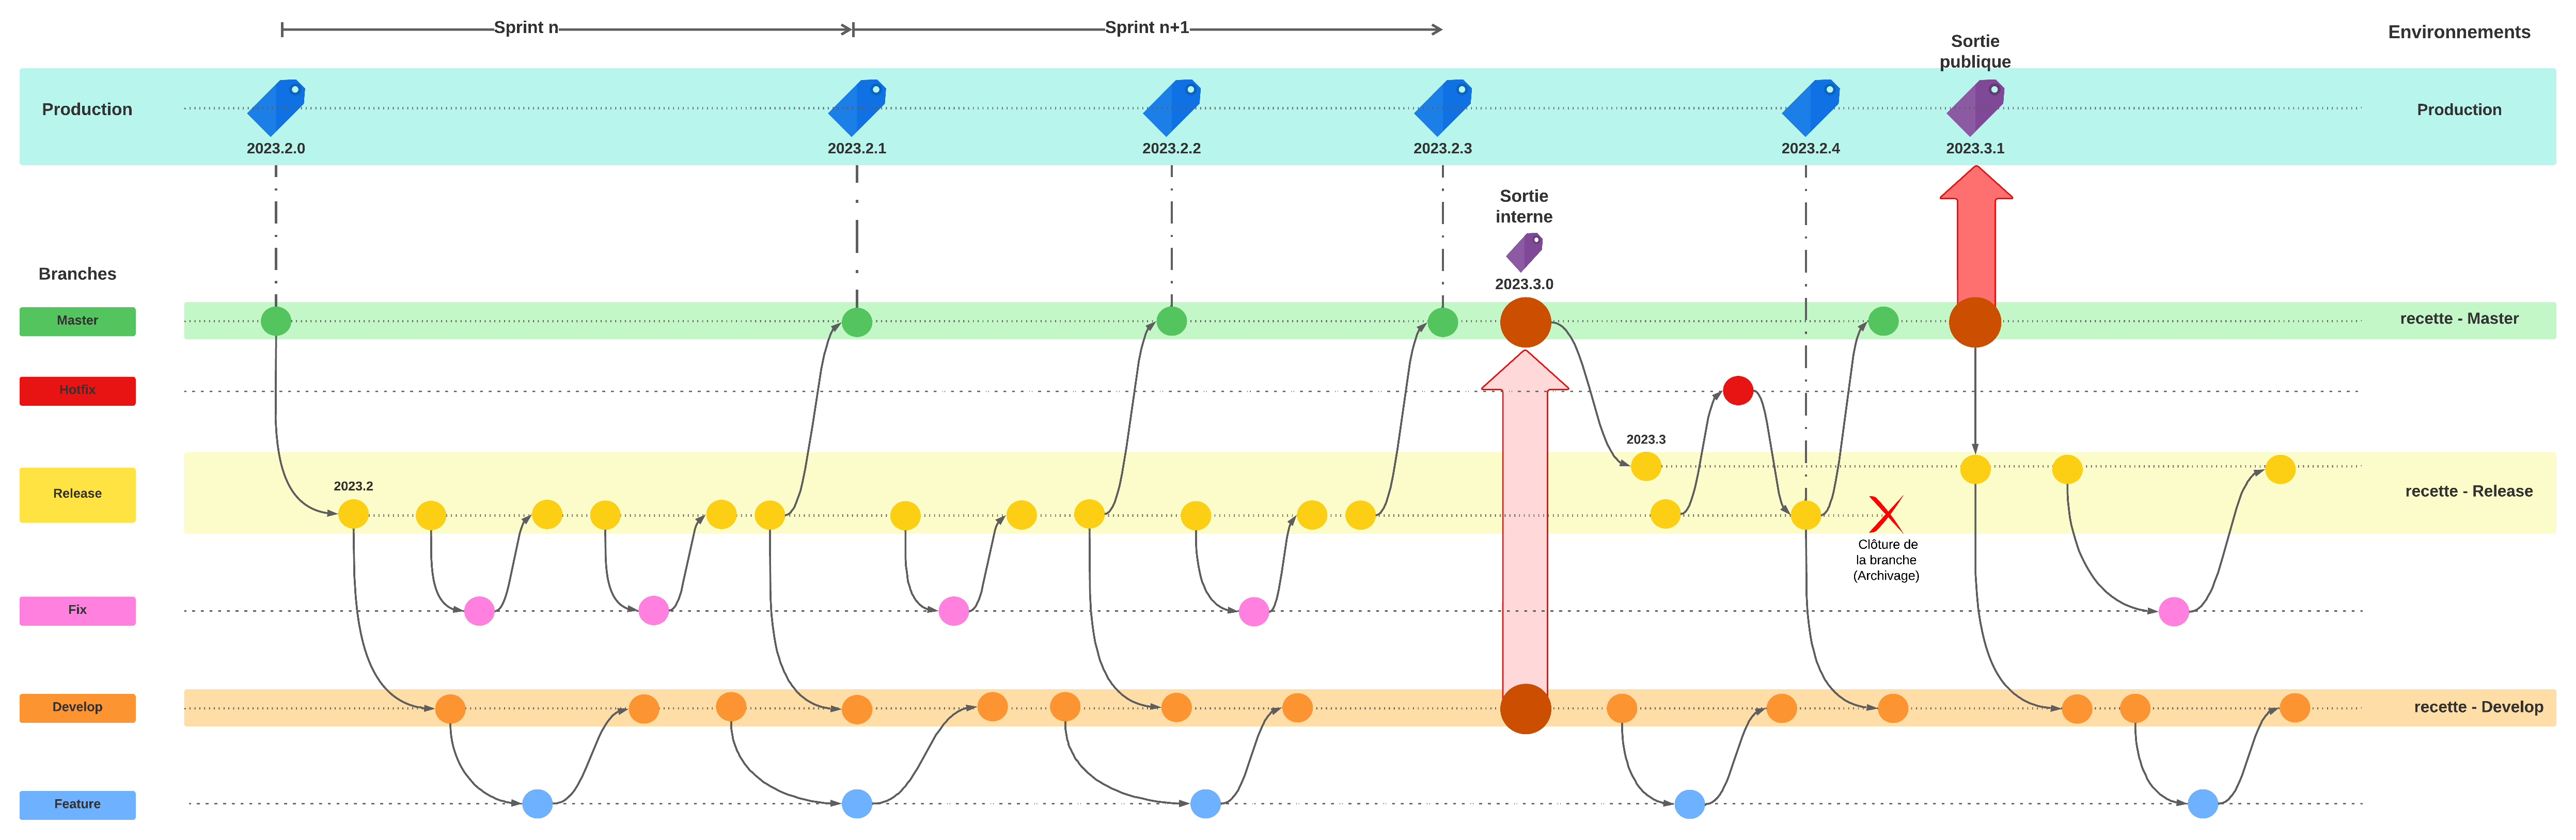
\includegraphics[width=\textwidth]{img/versioning-and-environments}
    \caption{Le schéma du versioning et des environnements.}
    \label{fig:versioning-and-environments}
\end{sidewaysfigure}

\begin{longtblr}[
    caption={Les caractéristiques des différents environnements.},
    label={tblr:environments}
    ]{
    hlines,vlines,
    rowspec={Q[m,font=\footnotesize\bfseries,gray9]*{5}{Q[m,font=\footnotesize]}}
    }
    Environnement    & {Pour quels                       \\ services} & Branches & {Type de \\ comits} & {Déploiement \\ TeamCity} \\
    {Dev pour chaque                                     \\ développeur} & Développeur & {Développeur \\ sandbox} &  & -- \\
    recette-develop  & {Le PO vérifie                    \\ les fonction-\\nalités}                                & develop             & feat                                                         & Auto                                                                      \\
    recette-releases & {Le PO vérifie                    \\ les corrections}                                    & releases/édition    & fix                                                          & Auto                                                                      \\
    recette-master   & {Autres                           \\ services                    \\ pour test \\ (direction, \\ marketing, \\ commerce \\ \dots)} & master              & {(env juste \\ avant la prod, \\ préproduction)}                     & {Manuel, \\ section master \\ dans TeamCity, \\ demande via \\ ticket MEP \\ à DevOps}     \\
    production       &                & tag & {Commit en \\ production \\ avec tag \\ \{numéro-édtion\}.\\\{numéro-increment\}} & {Manuel, \\ section \\ production \\ dans TeamCity, \\ demande via \\ ticket MEP \\ à DevOps}
\end{longtblr}